\documentclass{article}
\usepackage[utf8]{luainputenc}
\usepackage[T1]{fontenc}
\usepackage[a4paper,margin=0.75in, bottom=1in]{geometry}
\usepackage{listings}
\usepackage{courier}
\usepackage{amsmath}
\usepackage{amssymb}
\usepackage{enumerate}
\usepackage{graphicx}
\usepackage{hyperref}

\begin{document}
	
	\hrulefill
	\begin{center}
		\bfseries % Fettdruck einschalten
		\sffamily % Serifenlose Schrift
		\begin{huge}
			GTI: Grundlagen der Theoretischen Informatik
		\end{huge}\\
		\begin{Large}
			Sommersemester 2017, 3. Übungsblatt
		\end{Large}\\
		\begin{small}
			Valentin Wolf, Luis Herrmann; Tutor: Kristin Knorr; Mo 12:00-14:00
		\end{small}
		
		\vspace{-10pt}
	\end{center}
	\hrulefill
	
\section*{Aufgabe 1 - \textit{Regulär}}
	
Sei $A_L := (Q, \Sigma, s_0, \delta, F)$ der Automat, der die Sprache $L$ akzeptiert. Wir konstruieren einen nfa $N := (Q \cup \{s_{-1}\}, s_{-1}, \delta_N, Q)$, welcher von den akzeptierenden Zuständen $f\in F$ aus alle Zustände findet, von denen ein Endzustand nach $n: =|w|$ gelesenen Zeichen erreicht werden kann, wobei $w$ ein beliebiges Eingabewort ist. Da wir nicht die Menge aller akzeptierenden Zustände als Anfangszustand nehmen können, konstruieren wir einen zusätzlichen, vorgeschalteten Zustand $s_{-1}$, durch den alle akzeptierenden Zustände per $\epsilon$-Übergang erreicht werden können.

\begin{equation}
	\delta_N(q, a) = \begin{cases}
		F, &q = s_{-1} \land a=\epsilon\\
		\{p \in Q | \delta(p,b) = q\}, &\text{für } p \text{ beliebig}
	\end{cases}
\end{equation}

Die Idee ist nun, für ein Eingabewort eine parallele Berechnung durchzuführen. In der ersten Berechnung wird überprüft, ob das Eingabewort $w \in L$ ist, in der zweiten Berechnung wird die Menge aller Zustände im Automaten von $A_L$ gefunden, von denen nach Lesen von $|w|$ Zeichen ein Endzustand in $F$ erreicht werden kann. Offenbar ist ein Wort $w$ in $L_\text{half}$ gdw. sich der Automat $A_L$ nach Lesen von $n$ Zeichen in einem Zustand befindet, von dem aus ein akzeptierender Zustand in weiteren $n$ Schritten erreicht werden kann. Formal heißt das:
\begin{equation}
	w\in L_\text{half} \Leftrightarrow \delta^*(w,s_0) \in \delta_N^*(w,s_{-1})
\end{equation}
Wir können unseren Automaten $A_h := (Q_h,\Sigma,(s_0,s_{-1}),\delta_h, F_h)$, der $w \in L_\text{half}$ überprüft, also wie folgt als dfa konstruieren:
\begin{align}
	&Q_h = Q \times \mathcal{P}(Q \cup \{s_{-1}\}) &\delta_h((q,P),a) = (\delta(q,a),\bigcup_{p \in P} \delta_N(p,a)) &&F_h = \{ (p,P) \in Q_h | p \in P\}
\end{align}

Da ein dfa existiert, der die Sprache $L_\text{half}$ akzeptiert, ist diese regulär.

\section*{Aufgabe 2 - \textit{Vom nfa zum regulären Ausdruck}}

Algorithmische Berechnung:
\begin{enumerate}
	\item[$n = 0$:]
	
	\begin{tabular}{l|ccc}
		& $r$ & $s$ & $t$ \\\hline
		$r$ & $\epsilon \cup 0$  &  $0 \cup 1$ & \\
		$s$ & & $\epsilon \cup 0$ & $1$ \\
		$t$ & $1$ & $0$ & $\epsilon \cup 0$
	\end{tabular}
	\item[$n = 1:$]
	
	\begin{enumerate}[1.]
	\item $L_{ss}^1 = L_{ss}^0 \cup L_{ss}^0 (L_{ss})^0 L_{ss}^0 = (\epsilon \cup 0) \cup (\epsilon \cup 0)(\epsilon \cup 0) = 0^*$
	\item $L_{sr}^1 = L_{sr}^0 \cup L_{ss}^0 (L_{ss}^0)^* L_{sr}^0 = \emptyset$
	\item $L_{st}^1 = L_{st}^0 \cup L_{ss}^0 (L_{ss}^0)^* L_{st}^0 = 1 \cup (\epsilon \cup 0)(\epsilon \cup 0)^* 1 = 0^*1$
	\item $L_{rs}^1 = L_{rs}^0 \cup L_{rs}^0 (L_{ss}^0)^* L_{ss}^0 = (0 \cup 1) \cup (0\cup 1)(\epsilon \cup 0)^* (\epsilon \cup 0) = (0 \cup 1)0^*$
	\item $L_{rr}^1 = L_{rr}^0 \cup L_{rs}^0 (L_{ss}^0)^* L_{sr}^0 = \epsilon \cup 0$
	\item $L_{rt}^1 = L_{rt}^0 \cup L_{rs}^0 (L_{ss}^0)^* L_{st}^0 = (0 \cup 1 )(\epsilon \cup 0)^* 1 = (0\cup 1)0^*1$
	\item $L_{ts}^1 = L_{ts}^0 \cup L_{ts}^0 (L_{ss}^0)^* L_{ss}^0 = 0 \cup 0(\epsilon \cup 0)^* (\epsilon \cup 0) = 00^*$
	\item $L_{tr}^1 = L_{tr}^0 \cup L_{ts}^0 (L_{ss}^0)^* L_{sr}^0 = 1$
	\item $L_{tt}^1 = L_{tt}^0 \cup L_{ts}^0 (L_{ss}^0)^* L_{st}^0 = (\epsilon \cup 0 ) \cup 0(\epsilon \cup 0)^* 1 = \epsilon \cup 0 \cup 00^*1$
	\end{enumerate}

	\item[$n=2:$]
	\begin{enumerate}[1.]
	\item $L_{ss}^2 = L_{ss}^1 \cup L_{sr}^1 (L_{rr}^1 )^* L_{rs}^1 = 0^*$
	\item $L_{st}^2 = L_{st}^1 \cup L_{sr}^1 (L_{rr}^1)^* L_{rt}^1 = 0^*1$
	\item $L_{tt}^2 = L_{tt}^1 \cup L_{tr}^1 (L_{rr}^1)^* L_{rt}^1 = (\epsilon \cup 0 \cup 00^*1) \cup 1 (\epsilon \cup 0)^* (0\cup 1)0^* 1 = \epsilon \cup 0 \cup 00^*1 \cup 10^* (0 \cup 1)0^* 1$
	\item $L_{ts}^2 = L_{ts}^1 \cup L_{tr}^1 (L_{rr}^1 )^* L_{rs}^1 = 00^* \cup 1 (\epsilon \cup 0)^* (0 \cup 1)0^* = 00^* \cup 10^*(0\cup 1)0^* $
	\end{enumerate}

	\item[$n=3:$]
	\begin{equation}
		L_{ss}^3 = L_{ss}^2 \cup L_{st}^2 (L_{tt}^2)^* L_{ts}^2 = 0^* \cup 0^*1 (\epsilon \cup 0  \cup 00^*1 \cup 10^*(0\cup 1)0^*1 )^* (00^* \cup 10^*(0\cup 1)0^*)
	\end{equation}
	
	
\end{enumerate}


\section*{Aufgabe 3 - \textit{Nochmal nfa, dfa und regulärer Ausdruck}}

Wir konstruieren zunächst den äquivalenten dfa:

\begin{minipage}{\textwidth}
	\centering 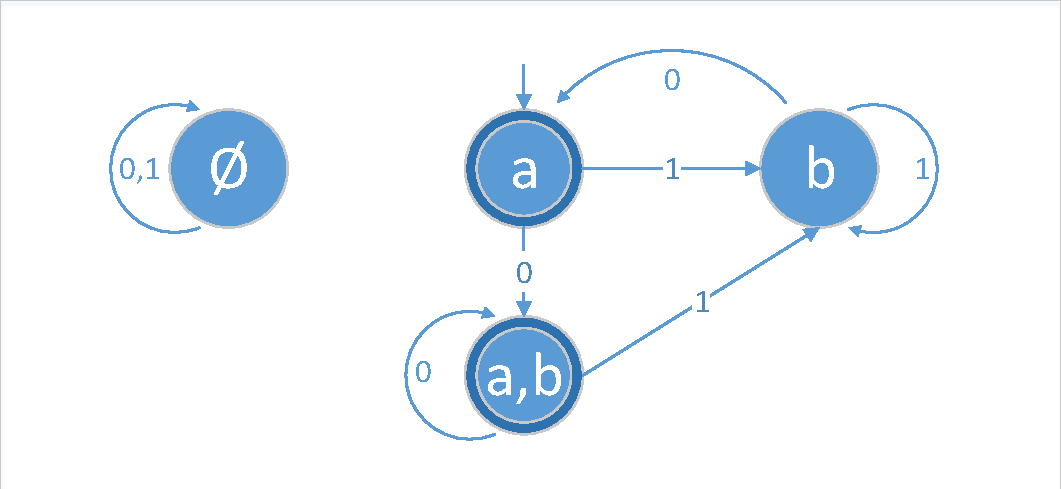
\includegraphics[width=0.6\textwidth,page=1,trim={2 2 2 4},clip]{dfas.pdf}
\end{minipage}

Dieser ist nun leicht zu minimalisieren. Zunächst halten wir fest, dass $\emptyset$ überflüssig ist, da dieser nicht erreicht werden kann. Dann betrachten wir als nächstes äquivalente Zustände: Offenbar gilt $\{a,b\} \equiv \{a\}$, denn $\delta^*(1w,\{a\}) = \delta^*(w,\{b\}) = \delta^*(1w, \{a,b\})$ und $\delta^*(0w,\{a\}) = \delta^*(w,\{a,b\}) = \delta^*(0w,\{a,b\})$, also gilt $\forall w \in \Sigma^* : \delta^*(w, \{a\}) \in F \Leftrightarrow \delta^*(w, \{a,b\}) \in F$ und wir haben Äquivalenz von $\{a\}$ und $\{b\}$ gezeigt. Weitere äquivalente Zustände existieren nicht.

\begin{minipage}{\textwidth}
	\begin{minipage}{0.5\textwidth}
		\centering
			\begin{tabular}{l|cc}
			& a & b\\\hline
			a & $X^\epsilon$  & \\
			a,b & / & $X^\epsilon$ \\
		\end{tabular}
	\end{minipage}
	\begin{minipage}{0.5\textwidth}
		\centering \includegraphics[width=\textwidth,page=2,trim={2 2 2 4},clip]{dfas.pdf}
	\end{minipage}
\end{minipage}

Es ist klar, dass der dfa genau die 0-1-Wörter akzeptiert, die nicht auf '1' enden, die zugehörige Sprache wird also durch den regulären Ausdruck $\epsilon \cup (0 \cup 1)^* 0$ beschrieben.

Rechnet man mit dem Algorithmus aus der Vorlesung, ist es etwas aufwendiger, den regulären Ausdruck der Sprache zu bestimmen:

\begin{enumerate}
	\item[$n=0$:]
	
	\begin{tabular}{l|cc}
		& a & b \\\hline
		a & $\epsilon \cup 0$ & 1 \\
		b & 0  & $\epsilon \cup 1$ \\
	\end{tabular}

	\item[$n=1$:]
	\begin{enumerate}[1.]
		\item $L_{aa}^1 = L_{aa}^0 \cup L_{aa}^0 (L_{aa}^0)^* L_{aa}^0 = (\epsilon \cup 0) \cup (\epsilon \cup 0)(\epsilon \cup 0)^*(\epsilon \cup 0) = 0^*$
		\item $L_{ab}^1 = L_{ab}^0 \cup L_{aa}^0 (L_{aa}^0)^* L_{ab}^0 = 1 \cup (\epsilon \cup 0)(\epsilon \cup 0)^*1 = 0^*1$
		\item $L_{ba}^1 = L_{ba}^0 \cup L_{ba}^0 (L_{aa}^0)^* L_{aa}^0 = 0 \cup 0(\epsilon \cup 0)^* (\epsilon \cup 0) = 00^*$
		\item $L_{bb}^1 = L_{bb}^0 \cup L_{ba}^0 (L_{aa}^0)^* L_{ab}^0 = (\epsilon \cup 1) \cup 0(\epsilon \cup 0)^* 1 = \epsilon \cup 1 \cup 00^*1$
	\end{enumerate}

	\item[$n=2$:]
	
	\begin{equation}
		L_{aa}^2 = L_{aa}^1 \cup L_{ab}^1 (L_{bb}^2)^* L_{ba}^1 = 0^* \cup 0^*1 (\epsilon \cup 1 \cup 00^*1)^* 00^*
	\end{equation}
	
	
\end{enumerate}


\section*{Aufgabe 4 - \textit{Minimalautomat}}

Wir benutzen den in der Vorlesung kennegelernten Algorithmus zum Minimieren von Automaten. Nach zwei Iterationsstufen werden keine neuen Zustandspaare mehr markiert und der Algorithmus terminiert somit. Es ergeben sich zwei Zustandspaare, für die kein Zeuge exisitert.

\begin{table}[h]
	\begin{tabular}{c|ccccc}
		& $s$ & $u$ & $v$ & $w$ & $x$\\\hline
		$u$ & $X^1$ &&&&\\
		$v$ &  $X^1$ & / &&&\\
		$w$ &  $X^2$ & $X^1$ &$ X^1$ &&\\
		$x$ &  $X^\epsilon$ & $X^\epsilon$ & $X^\epsilon$ & $X^\epsilon$ &\\
		$y$ & $X^\epsilon$ & $X^\epsilon$ & $X^\epsilon$ & $X^\epsilon$ & /\\
	\end{tabular}
\end{table}

Also gilt $u \equiv v$ sowie $x \equiv y$ und wir können den dfa wie folgt reduzieren:

\begin{minipage}{\textwidth}
	\centering \includegraphics[width=0.5\textwidth,page=3,trim={2 2 2 4},clip]{dfas.pdf}
\end{minipage}

\end{document}